\section{Experimentation}\label{sec:exp}

\subsection{Dataset and Setup}

Experiments use the Cranfield dataset provided with the assignment. The
collection contains 1400 documents, 225 queries, and relevance judgments in
\texttt{cran\_qrels.json}. Any document with a relevance position from 1 to 4 is
treated as relevant. Graded relevance for nDCG is computed as $5-\text{position}$,
so position 1 receives the highest gain and position 4 the lowest non-zero gain.

Two systems are compared:

\begin{itemize}
    \item \textbf{Baseline}: TF-IDF cosine ranking with the same preprocessing
    and inverted scoring index, but pseudo-relevance feedback disabled.
    \item \textbf{Improved}: the full implemented system with pseudo-relevance
    feedback enabled using one feedback document.
\end{itemize}

Both systems are evaluated over all 225 queries for $k=1$ to $10$. The reported
metrics are Precision@k, Recall@k, F0.5@k, Average Precision@k, nDCG@k, MAP@k,
MRR@k, and runtime.

\subsection{Quantitative Results}

Table~\ref{tab:main_results} compares the baseline and improved systems at
$k=10$. The improved system gives higher Precision, Recall, F0.5, MAP, and nDCG.
MRR is slightly lower, which means feedback sometimes changes the first relevant
document's rank even while improving the overall top-10 set.

\begin{table}[h]
\centering
\caption{Baseline and improved retrieval performance at $k=10$.}
\label{tab:main_results}
\begin{tabular}{lcc}
\hline
Metric & Baseline & Improved \\
\hline
Precision@10 & 0.2862 & 0.3182 \\
Recall@10 & 0.4207 & 0.4543 \\
F0.5@10 & 0.2930 & 0.3240 \\
MAP@10 & 0.3247 & 0.3639 \\
nDCG@10 & 0.4830 & 0.5091 \\
MRR@10 & 0.7759 & 0.7623 \\
\hline
\end{tabular}
\end{table}

\begin{figure}[h]
\centering
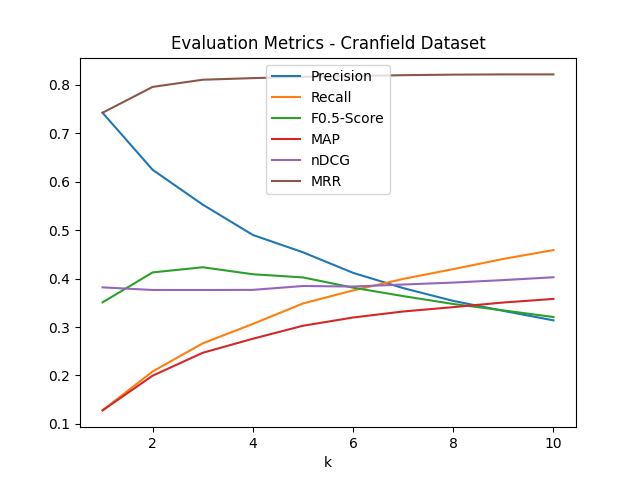
\includegraphics[width=0.72\linewidth]{../../template_code_part2/output/eval_plot.png}
\caption{Evaluation metrics of the improved system for $k=1$ to $10$.}
\label{fig:eval_plot}
\end{figure}

The improved system's full run produced Precision@1 of 0.6978 and Precision@10
of 0.3182. Recall increased from 0.1219 at $k=1$ to 0.4543 at $k=10$, which is
expected because more retrieved documents give the system more opportunities to
include relevant items. nDCG was 0.5633 at $k=1$ and 0.5091 at $k=10$, showing
that the system often places a relevant document first but still has ranking
errors lower in the top 10.

\subsection{Hypothesis Test and Runtime}

To test whether the improvement is consistent across queries, AP@10 was compared
query by query. The improved system had higher AP@10 for 110 queries, lower
AP@10 for 54 queries, and the same AP@10 for 61 queries. Ignoring ties, a
two-sided sign test gives $p \approx 1.46\times 10^{-5}$, so the AP@10
improvement is statistically meaningful under this paired non-parametric test.

The measured preprocessing, indexing, and baseline ranking time was about 1.65
seconds on the test machine. Once the index was built, the improved feedback
ranking pass over all queries took about 0.30 seconds. These numbers depend on
the machine, but they show that inverted-index scoring keeps the implementation
practical for the Cranfield collection.
